\title{Synthesizing Static Analyses from Examples}
\author{
        Martin Kellogg \\
        University of Washington
            \and
        Everett Maus\\
        Microsoft Corporation
}


\documentclass[10pt,conference]{IEEEtran}

\usepackage{graphicx}
\usepackage{myref}
\usepackage{booktabs}
\usepackage{url}
\usepackage{listings}

\begin{document}

\maketitle

\begin{abstract}

Constructing static analyses requires a great deal of
manual, expert programmer effort. Because of the large amount of
effort required to build a precise static analysis, custom analyses
are rarely deployed by developers, despite their potential
for finding bugs and verifying correctness. Compounding the problem,
the expert researchers who do design novel static analyses often
do not engineer their analyses to the level of practicality that
developers require. We propose a technique
for automatically synthesizing the implementation of analyses
from examples of the desired analysis in action,
reducing the effort required to design, build, and deploy static analysis
tools.

\end{abstract}

\section{Motivation}

A well-designed static analysis (or, equivalently, a type system or
abstract interpretation) can allow developers to find bugs in their
code quickly and with little manual effort, or even avoid entire
classes of errors by verifying that their code can never enter an
undesirable state. However, these benefits come at a cost---developing
such a static analyses requires an expert to spend a long time both
designing and implementing the static analysis (for instance, a static
analysis that checks the types of the arguments to a format string was
novel enough to be published at a recent top-tier software engineering
venue~\cite{format-string-checker}).  Worse, the cost to build such
static analyses means that many that are designed by the research
community are never engineered to the level of practicality and
precision that would be required to run on real-world code, so most
programmers never gain their benefits.

We propose to deploy state-of-the-art techniques from the domain of program
synthesis to allow programmers to specify a static analysis by providing
examples of the code that the analysis should and should not permit.
Our technique then synthesizes an abstract interpretation of the analysis,
which is then mechanically translated to an analysis framework like
the Checker Framework~\cite{checker-framework} or LLVM~\cite{lattner04:_llvm}.
A simple analysis could be specified
with just a few test cases (consider, for example, a function that needs to
be called with arguments that are related more precisely than a typical
type system would allow the programmer to express, like a pair of integers that
must sum to zero---with a few test cases and our technique, an analysis that
enforces this property could be run on an entire industrial codebase).
This will relieve the burden of actually building the infrastructure
required to deploy complex static analyses, so that specialized analyses
with the precision required of industrial-strength tools can be built without
requiring an intimate knowledge of the theory of abstract interpretation,
which will allow non-specialists (like industrial programmers) to easily
build new, customizable static analyses.

We envision a scenario like this: a developer or a researcher comes up with
a new static analysis. To test out their analysis today, they would need
to build the entire static analysis in an existing framework (like the Checker
Framework~\cite{checker-framework}). This requires them to: determine
the lattice and transfer functions used by their analysis (see \secref{ai}),
understand how
to use the framework they choose for implementation, write the implemention,
and finally to test and debug the implementation. Our proposed technique
shortcuts this process: it requires them only to determine the lattice
and then to write a series of examples of the analysis in action, which
should be equivalent to the test suite they would have to write anyway.
Then, they can apply the analysis to the code they care about, and any
place where it fails in practice (with either a false negative or a false
positive) can be added to the test suite from which the analysis
is generated. In this way, our approach allows analyses to be constructed
relatively cheaply and iterated on until they achieve the desired precision.

The technique we describe above requires several pieces:
\begin{enumerate}
\item A parser for annotated programs in the target language.
\item A tool that traverses the abstract syntax tree produced by 1) and
generates constraints on the transfer functions.
\item A tool that takes a lattice and a target language and produces
a set of \emph{sketches} (see \secref{synth}) of the transfer function.
\item A solver that takes the output of 2) and 3) and produces
a complete transfer function.
\item A framework for building static analyses that run on the target language.
\item A tool that translates the output of 4) into a static analysis built in
5).
\end{enumerate}

Off-the-shelf tools can be used for items 1), 4), and 5) above: many
languages support annotations~\cite{jsr308},
modern SMT solvers are fast on most queries~\cite{z3},
and frameworks for building static analyses exist in many common languages
(like the Checker Framework~\cite{checker-framework} for Java). Our tool
must provide 2), 3), and 6). We believe the most difficult parts to
get right (and therefore the most interesting research contribution)
will be in 2) and 3): designing the constraint generation tool and the
sketches so that they capture the static analysis the programmer intended
with a small number of test cases, we believe, is the most challenging
problem. Our proposal for this class therefore focuses on those parts,
leaving 6) as future work.

\section{Background}

\subsection{Abstract Interpretation}
\label{sec-ai}

\begin{figure}
 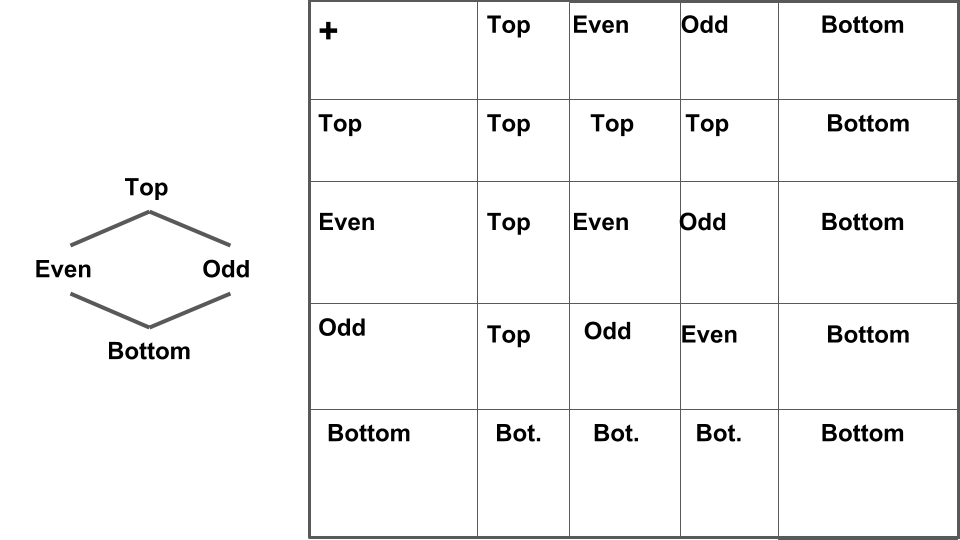
\includegraphics[width=\linewidth]{parity.png}
 \caption{A lattice of abstract domains and a transfer function
   for plus, for an abstract analysis that tracks the parity of
 a value.}
\label{fig-parity}
\end{figure} 

A static analysis can be formally modelled
as a lattice of \textit{abstract domains} and a set of \textit{transfer functions}
that transform abstract domains to other abstract domains when some
program operator is encountered~\cite{cousot77}. The analysis then proceeds by symbolically
interpreting the program being analyzed, replacing each concrete value with
an abstract domain determined by applying the transfer functions. An example
lattice and transfer function for the plus operator are given in Figure~1.
The analysis shown in Figure~1 is a parity analysis---it keeps track of
whether integers are even or odd. There are also two other possiblities:
the integer could be either even or odd (the ``top'' type) or it could
be \textit{both} even and odd---such as in dead code (represented by the
``bottom'' type). The lattice shows how these abstract domains are related,
with a subset relationship represented by the lines---any abstract domain
with a line going to another abstract domain higher in the lattice is a strict
subset of the higher abstract domain (so, for instance, top contains both
all even integers and all odd integers, so both even and odd are below it in the lattice).
The transfer function shows how the result of the plus operation is related
to its operands. We represent this as a matrix, with the top row and leftmost
column representing the abstract domains of the operands, and the interior
parts of the matrix representing the abstract domain of the result. So,
as an example, if $a$ is odd and $b$ is bottom, then $a + b$ is bottom,
because the entry for odd and bottom in the matrix is bottom.

\subsection{Synthesis}
\label{sec-synth}

The field of program synthesis uses SMT solvers to
automatically build programs based on a set of constraints provided
by the programmer. Modern SMT solvers, such as z3~\cite{z3}, are able
to solve equations involving millions of variables extremely quickly, despite 
the problem they solve (boolean satisfiabilty) being known to be NP-complete~\cite{cook71complexity}. 
These modern solvers allow the synthesis of, for example, memory models for modern architectures
in a few seconds from the architecture's litmus tests~\cite{bornholt17}.
Synthesis works by reducing the constraints provided by the user
(litmus tests, a formal specification, etc.) to a boolean satisfiability
problem, calling the solver, and then translating the result back into
a program. Because the search space for programs is so large, practical
synthesis techniques use \textit{sketches} of the solution to reduce
the search space. A sketch is an outline of the form of the answer,
such as a program with some expressions missing.

\section{Technical Approach}
\label{sec-tech}

\begin{figure}
 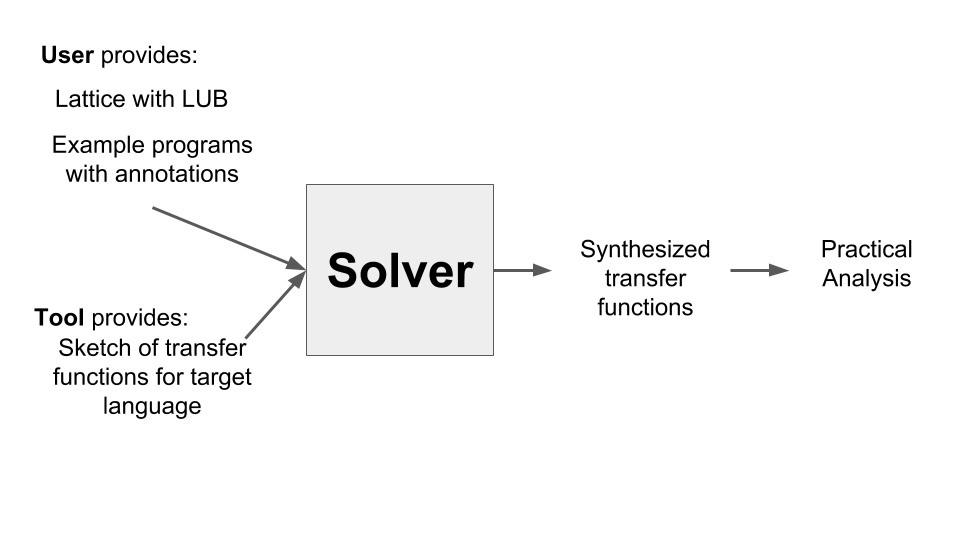
\includegraphics[width=\linewidth]{arch.png}
 \caption{The proposed architecture for the tool.
   Examples are translated to contraints and a sketch of the transfer function is built.
   These are passed to a solver, and then the resulting transfer function is translated into
 a practical analysis.}
\label{fig-arch}
\end{figure} 

Our proposed approach involves three steps.
First, translate examples of the static analysis on sample programs
(provided by the programmer)
into constraints on the transfer function and create
a sketch of the transfer functions for the target language.
Constraints are generated from annotated
code examples by traversing the abstract syntax tree of the
program.
Second, pass those constraints and the sketch to the solver;
the result of that solver call is a filled-in transfer
function. Finally, translate the produced transfer function
into an actual analysis that can be run by a programmer.
A diagram of this architecture is shown in \figref{arch}.

The lattice for the abstract analysis is provided by
the programmer, since it must be known to write the examples.
The examples are code snippets annotated with the
abstract domains (in the same way typed languages have type annotations).
Consider the example below, which is a sample example that a
programmer might write while building a parity analysis like the one
used as an example in \secref{ai}:

\begin{lstlisting}
@Even x = 2;
@Even y = 4;
@Even z = x + y;
\end{lstlisting}

The programmer must have already provided the names of the annotations
to the tool as part of the lattice.
Then, when this example is processed, the tool generates
the following \lstinline{smt2}~\cite{smt2} constraints:

\begin{lstlisting}
(assert (= (abstract-abstraction 2) @Even))
(assert (= (abstract-abstraction 4) @Even))
(assert (= (abstract-plus @Even @Even) @Even))
\end{lstlisting}

Each of these constraints corresponds to one of the statements in the
simple imperative program above. \lstinline{abstract-abstraction}
and \lstinline{abstract-plus} are defined in the sketch and define,
respectively, the abstraction function (i.e. the transfer function
for constants) and the transfer function for the plus operator.
The first two constraints indicate that both 2 and 4 are members of
the ``Even'' abstract domain. The last constraint indicates that
adding two even numbers produces another even number. Solving these
constraints results in a series of function definitions, which together
make up the transfer function. It is possible that the programmer's
examples might not completely specify the analysis. We believe that in
practice this will be solvable by observing the warnings produced by
the synthesized analysis and adding more test cases. However, ambiguity
can also be addressed at the tool level: once the solver returns a
candidate transfer function, a new solver call can be made that asks
the solver for another transfer function with the same properties (i.e.
that is still consistent with the examples) but which is \emph{not} the
transfer function it returned previously. If the result is unsatisfiable,
then we can conclusively say that there is no ambiguity; if not, one
can imagine a user-interface that asks the developer for help in
resolving the ambiguity by providing an example that disambiguates the
place that the two produced transfer functions differ.

This produced transfer function, along with the known lattice,
contains enough information to mechanically create the practical
analysis on top of a backend. Potential backends include frameworks like the
Checker Framework~\cite{checker-framework} (for Java)
or LLVM~\cite{lattner04:_llvm} (for C/C++). The backend chosen will
depend on the target language.

The main benefit of our approach is that it relieves the burden of
writing the transfer function from the programmer. The programmer
only needs to write a few slices of annotated code and to provide
the lattice. Instead of
needing to write a lot of code in a possibly unfamiliar framework
(i.e. the backend being used by our tool), the programmer only needs to
write test cases in the language being analyzed---which is the langauge
they are already working in! Further, actually writing the analysis
would require testing it, and our tool's input is exactly the test
cases a conscientious analysis developer would want to write.

\section{Implementation}

We propose to target the IMP programming language~\footnote{https://www.seas.upenn.edu/~cis500/current/sf/Imp.html}
during this course project, with the idea that we would be able to re-use the internals
(i.e. the code that calls the solver) if the project is successful in
a version of the tool that targetted a more practical language like Java.
We are choosing to use IMP because it's simple and we can avoid worrying
about the more complex details of a practical language. We are more interested
in determining whether it is possible to derive static analyses automatically
from examples at all, rather than building a production-quality tool.
We will use z3~\cite{z3} as our solver, and transform the IMP programs directly
into smt2 constraints using a modified IMP interpreter.
We will not
implement the last stage of our proposed approach, but rather stop with a
synthesized transfer function (there is also little practical value in building
a backend for IMP).

\subsection{Expected Challenges}

We anticipate that it will be difficult to produce constraints that allow
the solver to find a reasonable transfer. First, there is a danger that
the constraints will be too general, and that the produced transfer
function will be ambiguous. For that reason, we want to investigate
how many test cases we need to specify the correct transfer function
for several analyses (see the next section). This is the most important
concern that we have about this approach now. There is also a danger
that the produced transfer functions will overfit to the examples,
though. Consider the parity example in \secref{tech}. What if the solver
learns that 2 and 4 are members of the ``Even'' abstract domain, but
does not learn the more general rule for even numbers? Finding the
appropriate balance between asking the programmer for help (for instance,
we could ask the programmer to provide the abstraction function for
constants directly) and automatically inferring transfer functions
is our most pressing concern.

Related, we are also concerned that due to ambiguity in the provided
examples, the solver may produce an unsound transfer function.
As a pathological example, consider a transfer function where
everything goes to bottom. We would like to bias the solver
so that when it encounters ambiguity, it prefers a solution
closer to top. We mentioned in \secref{tech} that a possible solution
to the ambiguity issue is to iteratively call the solver, asking for
a different solution. We could then order the transfer functions
by how close they are to top (i.e. if one transfer function sends something
to bottom, but another sends it to top, select the one that sends it to top).
This is a inelegant solution that may make the
time required to run the tool infeasible, however, because
many solver calls could be required.
As part of our investigation, we will try to
determine if this actually is a problem when writing practical
analyses (or do a reasonable set of test cases prevent this?).

\section{Evaluation}
\label{sec-eval}

\begin{table}
\centering
 \begin{tabular}{l c c c c }
  
  Analysis & Test Cases & Precision & Recall & F-measure\\ 
  \midrule
  Parity0 & 4 & 0.46 & 0.46 & 0.46 \\
  Parity1 & - & - & - & - \\
  ... & - & - & - & - \\
  Sign0 & - & - & - & - \\
  Sign1 & - & - & - & - \\
  ... & - & - & - & - \\
  NPE0 & - & - & - & - \\
  NPE1 & - & - & - & - \\
  ... & - & - & - & - \\
  Range0 & - & - & - & - \\
  Range1 & - & - & - & - \\
  ... & - & - & - & - \\
 \end{tabular}
 \caption{Evaluation of synthesized transfer functions compared
 to ground truth transfer functions. Different analyses with
 the same name but a different number have the same ground truth
 but use a different set of test cases. The analyses are ordered
 by the number of test cases they used. Precision, recall, and
 F-measure are calculated in the standard way against the ground
 truth transfer function.}
 \label{tab-analyses}
\end{table} 

We will evaluate our approach by comparing the synthesized transfer
functions for several analyses to the ground truth accepted transfer
functions. The analyses we will consider are: a parity analysis,
a signedness analysis, a null-pointer analysis (using a version of
IMP augmented with a heap), and a range analysis, in that order.

\tabref{analyses} contains a skeleton of our proposed evaluation.
Each row in the table corresponds to a generated set of transfer functions.
For instance,
the row labeled ``Parity0'' states that it is a parity analysis
(from the name), that it was synthesized from 4 test cases,
and its precision, recall, and F-measure when compared to the ground
truth transfer functions were all 0.46. Because the parity analysis is only
relevant for integers, only the transfer functions on integer expressions
were considered.
The ground truth transfer functions were created manually by the authors,
but follow the established standards for their respective analyses.
Precision, recall, and F-measure were calculated following the standard
procedure: precision is the percentage of transfer function entries
in the synthesized transfer function that also appear in the ground truth,
recall is the percentage of transfer function entries in the ground truth
that appear in the synthesized transfer function, and F-measure is the
geometric mean of precision and recall.

\begin{table}
\centering
 \begin{tabular}{l c c c c }
  
  Function & Correct & Incorrect & Imprecise & Total\\ 
  \midrule
  Plus & 7 & 0 & 9 & 16 \\
  Minus & 6 & 0 & 10 & 16 \\
  Times & 7 & 3 & 6 & 16 \\
  Divide & 9 & 0 & 7 & 16 \\
  Mod & 8 & 0 & 8 & 16 \\
  Negate & 2 & 0 & 2 & 4 \\
  \midrule
  Total & 39 & 3 & 42 & 84 \\
 \end{tabular}
 \caption{Breakdown of the results of synthesizing transfer functions
 for a parity analysis from just four simple test cases. Correct is number
 of entries in the matrix that match the ground truth transfer function
 exactly; Incorrect is the number that do not match and are unsound;
 Imprecise is the number that do not match, but are still sound. The
 precision/recall in Table I can be calculated by dividing
 the Correct column by the Total column.}
 \label{tab-parity0}
\end{table}

\begin{table}
\centering
 \begin{tabular}{l c c c c }
  
  Function & Correct & Incorrect & Imprecise & Total\\ 
  \midrule
  Plus & 5 & 0 & 11 & 16 \\
  Minus & 5 & 0 & 11 & 16 \\
  Times & 3 & 0 & 13 & 16 \\
  Divide & 8 & 0 & 8 & 16 \\
  Mod & 7 & 0 & 9 & 16 \\
  Negate & 1 & 0 & 3 & 4 \\
  \midrule
  Total & 29 & 0 & 55 & 84 \\
 \end{tabular}
 \caption{Equivalent table to Table II, but for an
 analysis that ``always goes to top''---meaning that every
 transfer function loses all precision.}
 \label{tab-top}
\end{table}

Because of these definitions of precision and recall, the
precision and recall will always be the same: we are actually just counting how
many entries in the transfer function matrix are identical. To further break
down how precise the ``parity0'' analysis is, consider \tabref{parity0}, which breaks
down each of the relevant transfer functions by the number of exactly correct
entries, the number of incorrect entries (i.e. unsound entries), and the
number of imprecise entries (i.e. entries that are sound but not as precise
as they could be). \tabref{top} shows the same table for an analysis whose
transfer functions are always top; this analysis is sound but not precise.
The generated transfer function gets 10 more cases correct, but also gets
three cases incorrect. That we are able to get several more cases correct,
even though we introduce a bit of unsoundness, with just four test cases
is encouraging. By adding more tests, we expect to improve these numbers.
The tests used to generate the analysis are shown in the Appendix.

The generated transfer functions also include transfer functions for
boolean expresssions, which are all sound but not particularly precise,
since they are mostly unconstrained. In addition, an abstraction function
is synthesized; it is not correct, because it abstracts every integer but 1
to be even. We are considering making the abstraction function an input to
the tool.

Our goal is to achieve a perfect match to the correct transfer function
on at least the parity analysis.
Determining how to reach that goal---how many test cases are required, how
we can bias the solver away from incorrect results---will be our goals
for the remainder of the project.
Since this is exploratory research, our primary goal here
is to just show that this is possible, not to demonstrate that our tool
is superior to the state of the art in any way. That will come later;
see \secref{fw}.

\section{Related Work}

There is a large body of work on abstract interpretation and its relationship
with other, similar static analysis techniques, which is far
too extensive to cover here.
For a sample, see Cousot and Cousot~\cite{cousot14}.
The mathematical framework provided by abstract interpretation is sufficiently
general to express most static analyses, including type systems.
As far as we are aware, this work is the first attempt to automatically
create abstract interpretations from a set of examples, but there is a
large body of prior work that makes building static analysis tools easier.
(whether they are based directly on abstract interpretation or not).
The Checker Framework makes building type systems for Java easier
by providing a framework for type system designers~\cite{checker-framework};
because types are an abstract interpretation, the Checker Framework
is a framework for designing and building abstract interpretations.
IKOS is a framework for developing static analyses directly based on
abstract interpretations, developed by NASA for verifying flight
controllers~\cite{ikos}. Modern compilers use a framework for building
the dataflow analyses they use to perform optimizations and code generation
~\cite{lattner04:_llvm}; these dataflow analyses, too, can be viewed as
abstract interpretations. The current state of the art in industry is to
utilize domain specific query languages to describe static analyses, such as 
Semmle's QL, a datalog variant~\cite{semmle-ql-primer}.
These frameworks and others like them make it easier and faster to develop analyses, but 
building a precise, sound analysis still requires an expert.  Our tool 
aims to remove that requirement by automating the development of analyses; 
we could target our tool to generate code that runs in any of these frameworks.

Previous work on abstract interpretation has considered its relationship
with SAT/SMT solvers, which our approach relies on. Brain et al. characterized
DPLL(T), the main algorithm upon which modern SAT/SMT solvers are built,
as an abstract interpretation~\cite{brain2013abstract}. By calling out to
an SMT solver as part of the transfer function, Jiang et al. are able to
improve the refinements made by their abstract
interpretations~\cite{jiang2017block}. The PAGAI static analyzer uses
an SMT solver to more precisely refine path conditions~\cite{pagai}.
While all of these results combine abstract interpretations with
an SAT or SMT solver in some way, none actually use the solver to
synthesize the abstract interpretation.

Counterexample-guided abstraction refinement (CEGAR) is a general technique
for improving verification results~\cite{cegar}. This technique can be
viewed as using a solver to refine an abstract interpretation into a
more precise abstract interpretation, but we are not aware of any
uses of the technique which generate an abstract interpretation from
only user-provided examples. CEGAR has been used in many contexts,
including model checking~\cite{clarke2003counterexample},
test generation~\cite{beyer2004},
and stability analysis~\cite{prabhakar2016counterexample}.

A similar domain is inferring invariants. Verifying a program is straightforward
(and can be mechanized~\cite{hoare69}) if inductive invariants are supplied for
each loop or recursive function, and generating these invariants is
known to be a synthesis problem. Recent work has focused on learning
invariants via a counter-example guided approach~\cite{garg2014ice} or
on guessing invariants via an efficient random search algorithm and then
checking whether they are correct~\cite{sharma2016invariant}.
These approaches still require the programmer to specify the correctness
properties of the system formally; our tool allows developers to specify
the analysis they need with examples. In practice, developers write
test cases like the ones our tool requires, but rarely formally specify
the properties of their systems.

Our approach relies on example-driven synthesis, which has been effectively
applied in other domains. Microsoft's Excel spreadsheet tool can automatically
synthesize programs to transform user input based on a few examples
provided by the user using FlashFill~\cite{flashfill}. Bornholt and
Torlak used litmus tests to synthesize memory models for complex architectures
like x86 and PowerPC~\cite{bornholt17}. Perelman et al. developed a general
framework for synthesizing programs from test cases~\cite{perelman2014test}.
These approaches (and ours) share a general framework: the user provides
some examples of what they are trying to accomplish, and a program
(whether it manipulates a spreadsheet, models the memory architecture of
a processor, or implements an abstract interpretation) is produced
automatically by a solver. Our technique extends approaches like these
to a promising new domain: abstract analyses.

\section{Future Work}
\label{sec-fw}

A conference-length paper on this topic would extend the tool to operate
on Java programs, with the final goal being the replication of
existing Checker Framework checkers using only those checkers'
test suites. This would require building more
complex transfer functions---and probably would require
a meta-sketching approach~\cite{metasketching} which tries several levels of
sketches for the transfer functions (moving from refining only the result of the expression, to
refining multiple variables, to a flow-sensitive refinement, etc.).
This would also require implementing the last stage of the tool, which
translates the synthesized transfer function into a Checker Framework
checker or some other backend. Getting this whole pipeline working would,
we think, be an interesting research contribution, but we are less
confident that the approach is feasible at all, so we intend to start
by validating whether we can produce transfer functions that are
similar to what a human might write before we worry about translating
them into practical analyses.

\section{References}

\begingroup
\renewcommand{\section}[2]{}%

% The following two commands are all you need in the initial runs of
% your .tex file to produce the bibliography for the citations in your
% paper.
\bibliographystyle{plain}
\bibliography{genprog-bib/merged}
% You must have a proper ``.bib'' file
% and remember to run:
% latex bibtex latex latex
% to resolve all references
%
% ACM needs 'a single self-contained file'!
%
\endgroup

\appendix

This appendix contains the test cases used to generate the ``parity0''
analysis discussed in \secref{eval}. The test cases are very simple and
were chosen for convenience.

\begin{lstlisting}
add_evens.imp:
        x = @Both read_int();
        @Even y = 2;
        @Even z = 2 * x;
        return @Even y + z;

add_evens_loop.imp:
        lc = read_int();
        @Even y = 0;
        while (0 < lc){
            @Even y = y + (@Even 2);
            lc = lc -1;
        }
        return y;

if_merge.imp:
        x = @Both read_int();
        y = x;
        if(x < 10) {
            @Odd y = 1;
        } else {
            @Even y = 2;
        }
        return y;

while_merge.imp:
        x = @Both read_int();
        y = x;
        while(0 < x) {
            x = x - @Odd 1;
            @Even y = 2 * y;
        }
        return y;

\end{lstlisting}

\end{document}
This is never printed
